\chapter{Anvendelsesgrænsetilstand}
I det følgende afsnit bestemmes anvendelsesgrænsetilstanden for tilbygningen til Strøybergs Palæ. Ud fra anvendelsesgrænsetilstanden kan det vurderes, om tilbygningen har tilstrækkelig små deformationer til, at dimensionerne kan godtages. 
\newline \indent{     }  Jævnført Eurocode 1993, afsnit 7.2, beregnes anvendelsesgrænsetilstanden kun for én variabel last, hvilken vælges til at være vindlasten. Derfor er der udregnet nye reaktioner for konstruktionen, som er vist på Figur \ref{fig:snitanvendelse}. Udregningerne findes i Bilag F punkt 7. 

\section{Momentligninger}
Ved udbøjning skal bjælkens differentialligning anvendes, og derfor skal momentligningen for hvert snit bruges. Udbøjningen beregnes ud fra hovedkonstruktionens stålstænger, hvor der laves fem snit, som vist på Figur \ref{fig:snitanvendelse}. Dog ses der bort fra den højre del af konstruktionen, og dermed er det kun snit 1-3 der anvendes.

\begin{figure}[H]
	\centering
	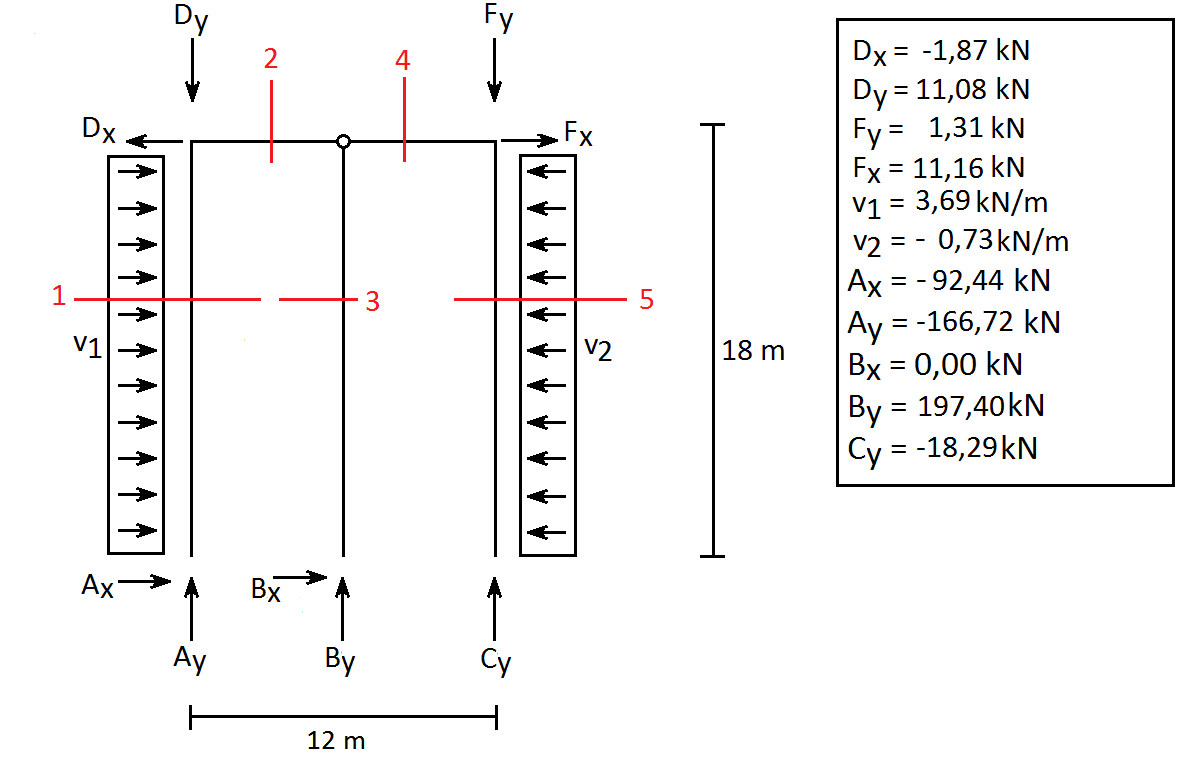
\includegraphics[width=0.9\textwidth]{billeder/snitanvendelse.png}
	\caption{Snit for statisk system kun med vindlast}
	\label{fig:snitanvendelse}
\end{figure}

Nedenfor er vist et eksempel på, hvordan momentligningen regnes for snit 1. Alle beregningerne af snitkræfterne findes i Bilag F punkt 8.
\newline
\newline
\textbf{Snit 1: 0 m < $x_1$ < 18 m}
\newline
Fritlegemediagrammet for snit 1 ses på Figur \ref{fig:snitetan}.
\begin{figure}[H]
	\centering
	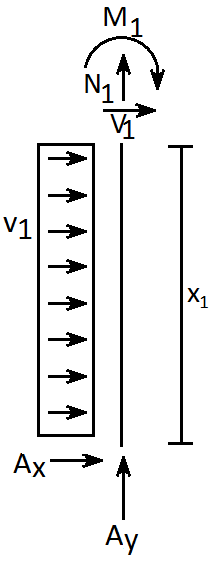
\includegraphics[width=0.3\textwidth]{billeder/asnitet.png}
	\caption{Snit 1}
	\label{fig:snitetan}
\end{figure}
\begin{equation}
	\ALN{\text{ }}: 0 = M_1 + A_x x_1 + v_1x_1 \frac{x_1}{2} \leftrightarrow M_1(x_1)= {-A_x x_1-\frac{1}{2}v_1x_1^2}
\end{equation}

Følgende momentligninger fås for snit 1, 2 og 3, og disse kaldes $M_1$, $M_2$ og $M_3$:
\begin{equation}
	M_1(x_1)= -A_x x_1-\frac{1}{2}v_1x_1^2 = v''EI
\end{equation}

\begin{equation}
	M_2(x_2)= -v_1 \cdot 162 \text{m}^2 - A_x \cdot \SI{18}{m} + A_yx_2 - P_1y x_2^2 = v''EI
\end{equation}

\begin{equation}
	M_3(x_3)= B_xx_3 = v''EI
\end{equation}

\section{Bjælkens differentialligning}
Da det statiske system for tilbygningen til Strøybergs Palæ er statisk bestemt, er det den anden ordens afledede, som anvendes for at bestemme udbøjningerne.

For $M_1$ bestemmes nu den første afledede $\alpha_1$ og anden afledede $u_1$: %Her vises integration%
\begin{equation}
	\int \frac{M_1(x_1)}{EI} dx_1 = \int \frac{-A_x x_1 - \frac{1}{2}\cdot v_1 x_1^2}{EI} dx_1
	\leftrightarrow \alpha_1(x_1) = \frac{-\frac{1}{2} A_x x_1^2 - \frac{1}{6}  v_1  x_1^3 }{EI} + k_1
\end{equation}

\begin{equation}
	\int \alpha_1(x_1) dx_1 = \int \frac{-\frac{1}{2} A_x x_1^2 - \frac{1}{6} v_1 x_1^3}{EI} + k_1 dx_1 \leftrightarrow
	u_1(x_1) = \frac{-\frac{1}{6} A_x x_1^3 - \frac{1}{24} v_1x_1^4 }{EI} + k_1 x_1 + k_2
\end{equation}

Det samme gøres for $M_2$ og $M_3$, hvilket giver følgende funktioner for den første og anden afledede: 
\newline
\newline
$M_2$:
\begin{equation}
	\alpha_2(x_2) = \frac{-v_1 \cdot 162 \text{m}^2 \cdot x_2 - A_x \cdot 18 \text{m} \cdot x_2 + \frac{1}{2} A_y x_2^2 - \frac{1}{2}P_1y x_2^2}{EI} + k_3
\end{equation}
	
\begin{equation}
	u_2(x_2) = \frac{-v_1 \cdot 81 \text{m}^2 x_2^2 - A_x \cdot 9 \text{m} \cdot x_2^2 + \frac{1}{6} A_y x_2^3 - \frac{1}{6} P_1y x_2^3}{EI} + k_3 x_2 + k_4
\end{equation} 
\newline
\newline
$M_3$:
\begin{equation}
\alpha_3(x_3) = \frac{1}{2}\frac{B_x x_3^2}{EI} + k_5
\end{equation}

\begin{equation}
u_3(x_3) = \frac{1}{6} \frac{B_x x_3^3}{EI} + k_5 x_3 + k_6
\end{equation}

Ved integrering af ligningerne giver dette 6 ligningner med 6 ubekendte konstanter. Disse bestemmes ved at opstille 6 randbetingelser for det statiske system: 

\begin{itemize}
	\item[-] $u_1(0)=0$: Der kan ikke ske en udbøjning ved understøtningen
	\item[-] $\alpha_1(h)$=$\alpha_2(0)$: Vinkeldrejningen mellem bjælke 1 og 2 skal være ens
	\item[-] $u_1(h)$=$u_3(h)$: Udbøjningen for bjælke 1 og 3 er ens i højden $h$
	\item[-] $u_2(0)$=0: Da vinkeldrejningen for bjælke 1 og 2 er ens, bliver vinklen mellem disse $90^{\circ}$, og udbøjningen er derfor 0
	\item[-] $u_2(l)$=0: Da vinkeldrejningen for bjælke 2 og 3 er ens, bliver vinklen mellem disse $90^{\circ}$, og udbøjningen er derfor 0
	\item[-] $u_3(0)$=0: Der kan ikke ske en udbøjning ved understøtningen
\end{itemize}

De opsatte randbetingelser løses, og de 6 konstanter får værdierne: 
\begin{itemize}
	\item[-] $k_1 = -0,\!14$
	\item[-] $k_2 = 0$
	\item[-] $k_3 = -0,\!02$
	\item[-] $k_4 = 0,\!00$
	\item[-] $k_5 = -0,\!10$
	\item[-] $k_6 = 0,\!00$
\end{itemize}

Udregningerne for konstanterne findes i Bilag F punkt 9.
\newline
\newline 
Konstanterne indsættes nu i formlerne for $u_1(x_1)$, $u_2(x_2)$ og $u_3(x_3)$, og ud fra de nye funktioner kan udbøjningen bestemmes (se Figur\ref{fig:udboj}).
\begin{equation}
u_1(18m) = \SI{-1762,89}{mm}
\end{equation}

\begin{equation}
u_2(3m) = \SI{-24,92}{mm}
\end{equation}

\begin{equation}
u_3(18m) = \SI{-1762,89}{mm}
\end{equation}

\begin{figure}[H]
	\centering
	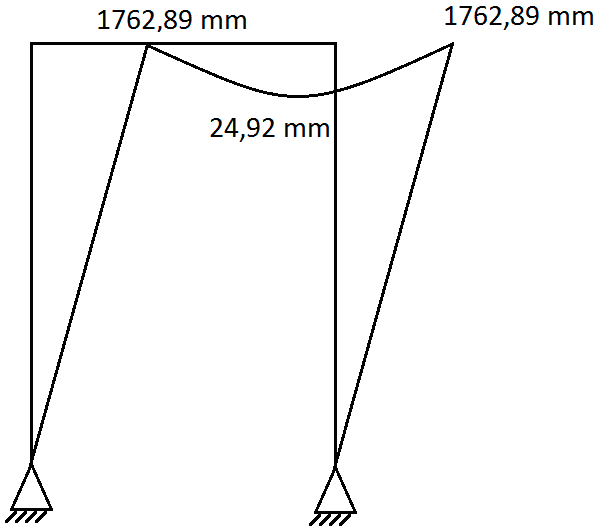
\includegraphics[width=0.4\textwidth]{billeder/udbog.png}
	\caption{Udbøjningskurve}
	\label{fig:udboj}
\end{figure}

Disse udbøjninger skal nu sammenlignes med de anbefalede udbøjningsværdier for en bærende konstruktion, som findes i Eurocode 1993, afsnit 7.2. 

Maksimal vandret udbøjning: 
\begin{equation}
\frac{h_3}{500}
\\
\frac{18000 \text{mm}}{500} = \SI{36}{mm}
\end{equation}

Maksimal lodret udbøjning
\begin{equation}
\frac{l}{400}
\\
\frac{6000 \text{mm}}{400} = \SI{15}{mm}
\end{equation}

Her fås, at de vandrette udbøjninger for stængerne 1 og 3 overskrider de anbefalede værdier med næsten faktor 50, mens den lodrette udbøjning er næsten dobbelt så stor som den anbefalede. De lodrette udbøjninger er meget voldsomme, og må anses at være urealistiske, hvorfor der må være en fejl i beregningerne. Grundet tidsnød har det ikke været muligt at finde frem til fejlen i udregningerne, men i stedet er der sammenlignet med udbøjningen for en fast indspændt bjælke, for at få et bedre estimat for, hvor stor udbøjningen må være for stængerne 1 og 3. 
\newline \indent{     }  Her anvendes udbøjningsformlen for en fast indspændt bjælke:
\begin{equation}
u(l)=\frac{1}{8} \frac{ql^4}{EI}
\end{equation}

Her sættes $q$ til en karakteristisk vindlast på 3,68 $\frac{\text{N}}{\text{mm}}$ og $l$ til 18.000 mm. Så fås udbøjningen til: 
\begin{equation}
u(18) = \frac{1}{8} \frac{3,69\frac{\text{N}}{\text{mm}} \cdot (18000 \text{mm})l^4}{0,21 \cdot 10^6 \cdot 458,5 \cdot 10^4} \leftrightarrow u(18) = \SI{501,52}{mm}
\end{equation}

Udbøjningen for stængerne 1 og 3 bør derfor maksimalt være 501,52 mm, hvilket er ca. 1/3 af den først beregnede. Denne beregning kan dog ikke bruges, da der ikke er tale om en fast indspændt bjælke, men blot give et estimat, og her kan denne støtte projektgruppens teori om, at der er en fejl beregningerne af udbøjningen for stang 1 og 3.

\section{Delkonklusion}
Med udgangspunkt i Lokalplan 1-1-107 er tilbygningens størrelser og dimensioner bestemt. Hertil er der opstillet et statisk system, og der er valgt at indsætte tre stålrammer, hvor der  dimensioneres efter den midterste ramme.
\newline \indent{     }  Tilbygningens stålprofiler er dimensioneret ud fra ståltype S235 med profil nr. 450, samt ud fra de permanente og variable laster, der virker på tilbygningen; egenlast, jordlast, vindlast, snelast og nyttelast. Ud fra disse laster er der opstillet én lastkombination, som er den dimensionsgivende i denne rapport. Der skal dimensioneres efter det mest kritiske tilfælde, og her blev tilfældet hvor vindlasten er den dominerende variable last valgt til at være den mest kritiske, hvorfor brud- og anvendelsesgrænsetilstanden er bestemt ud fra denne lastkombination. 
\newline \indent{     }  Gennem beregningerne for brudgrænsetilstanden kan det konkluderes, at tilbygningen har en tilstrækkelig bæreevne, da spændingerne for det statiske system ikke overskrider den regningsmæssige flydespænding på 204,54 MPa, idet der fås en maksimal spænding på 100,51 MPa.
\newline \indent{     }  Anvendelsesgrænsetilstanden for tilbygningen blev udregnet, og her kan det konkluderes, at udbøjningen for tre af konstruktionens stålstænger overskrider de anbefalede værdier fra Eurocode 1993. Den vandrette udbøjning var på 1762,89 mm, mens den lodrette var på 24,92 mm og derfor vil konstruktionen ikke kunne dimensioneres efter det statiske system. Her vil det dog være muligt, at sætte flere rammer i tilbygningen, for på den måde at mindske udbøjningen mellem hver af stålstængerne.
